\section{Ejercicios}

\subsection{Ejercicios de construcción - Pappus}

\begin{section-exercise}
    Aplicar el teorema de Pascal al hexágono $ABCDEF$. \hspace{1cm}
    \begin{tabular}{|c|c|c|}
        \hline
        \ \ \ \ && \\\hline
        &\ \ \ \ & \\\hline\hline
        &&\ \ \ \ \\\hline
    \end{tabular}
    \vspace*{\fill}
    \begin{figure}[H]
        \centering
        
%dash pattern=on 5pt off 2pt
%[fill = white, rounded corners = 5pt, inner sep=0.8pt]
\begin{tikzpicture}[scale = 1.2]
    \clip(-7.18,-0.99) rectangle (4.94,8.68);
    \draw [line width=1.2pt] (-3.5,4.81) circle (2.98cm);
    \begin{scriptsize}
        \normalsize
        \fill [color=black] (-4.5,7.62) circle (2.5pt);
        \draw[color=black] (-4.75,7.97) node {$A$};
        \fill [color=black] (-2.24,2.11) circle (2.5pt);
        \draw[color=black] (-1.96,1.72) node {$B$};
        \fill [color=black] (-5.84,2.97) circle (2.5pt);
        \draw[color=black] (-6.26,2.86) node {$C$};
        \fill [color=black] (-0.91,3.34) circle (2.5pt);
        \draw[color=black] (-0.54,3.22) node {$D$};
        \fill [color=black] (-0.52,4.85) circle (2.5pt);
        \draw[color=black] (-0.13,5.03) node {$E$};
        \fill [color=black] (-0.72,5.86) circle (2.5pt);
        \draw[color=black] (-0.4,6.13) node {$F$};
    \end{scriptsize}
\end{tikzpicture}
    \end{figure}
    \vspace*{\fill}
\end{section-exercise}

\newpage
\begin{section-exercise}
    Aplicar el teorema de Pappus, sabiendo que
    \begin{tabular}{|c|c|c|}
        \hline
        B & C & A\\\hline
        D & E & F\\
        \hline \hline
        &&\\
        \hline
    \end{tabular}
    \vspace*{\fill}
    \begin{figure}[H]
        \centering
        
%dash pattern=on 5pt off 2pt
%[fill = white, rounded corners = 5pt, inner sep=0.8pt]
\begin{tikzpicture}[scale = 1.2]
    \clip(-7.18,-0.99) rectangle (4.94,8.68);
    \draw [line width=1.2pt] (-3.5,4.81) circle (2.98cm);
    \begin{scriptsize}
        \normalsize
        \fill [color=black] (-4.5,7.62) circle (2.5pt);
        \draw[color=black] (-4.75,7.97) node {$A$};
        \fill [color=black] (-2.24,2.11) circle (2.5pt);
        \draw[color=black] (-1.96,1.72) node {$B$};
        \fill [color=black] (-5.84,2.97) circle (2.5pt);
        \draw[color=black] (-6.26,2.86) node {$C$};
        \fill [color=black] (-0.91,3.34) circle (2.5pt);
        \draw[color=black] (-0.54,3.22) node {$D$};
        \fill [color=black] (-0.52,4.85) circle (2.5pt);
        \draw[color=black] (-0.13,5.03) node {$E$};
        \fill [color=black] (-0.72,5.86) circle (2.5pt);
        \draw[color=black] (-0.4,6.13) node {$F$};
    \end{scriptsize}
\end{tikzpicture}
    \end{figure}
    \vspace*{\fill}
\end{section-exercise}




\newpage
\subsection{Ejercicios de perspectiva - Desargues}

\begin{section-exercise}
    Encuentre, con la ayuda de una regla, el punto y la recta para los cuales los triángulos \theTriangle{ABC} y \theTriangle{XYZ} están en perspectiva.

    \vspace*{\fill}
    \begin{figure}[H]
        \centering
        \definecolor{ttqqcc}{rgb}{0.33,0.33,0.33}
%dash pattern=on 5pt off 2pt
%[fill = white, rounded corners = 4pt, inner sep = 1pt]
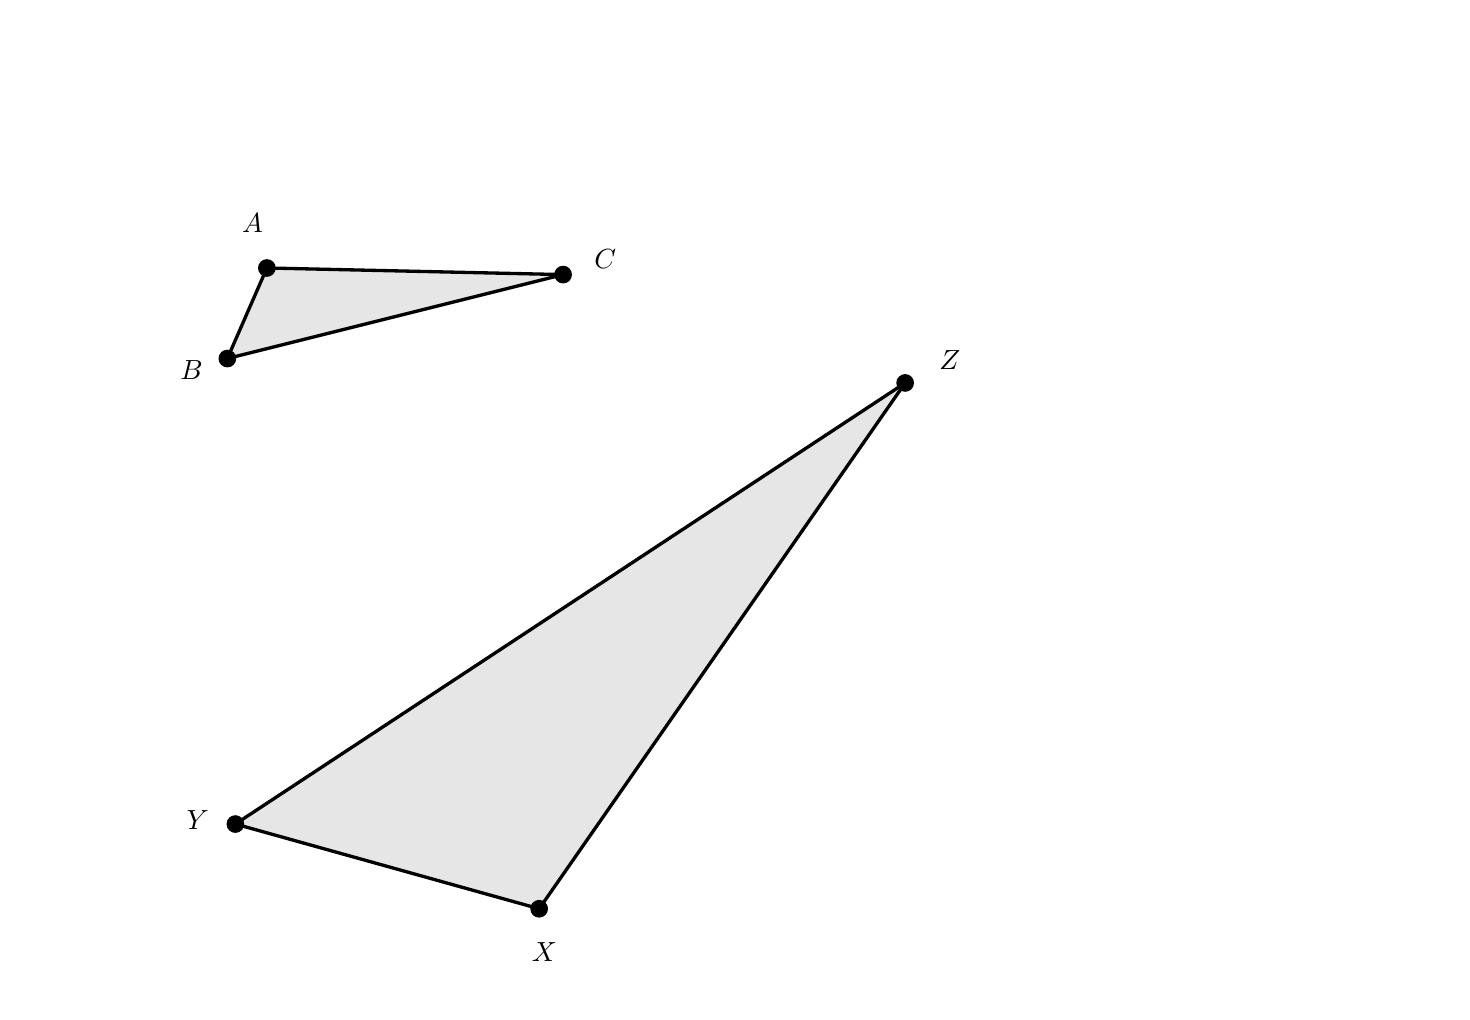
\begin{tikzpicture}[scale = 0.2]
    \clip(-20.65,-28.57) rectangle (69.12,32.66);
    \fill[line width=0pt,color=ttqqcc,fill=ttqqcc,fill opacity=0.15] (-5.46,17.4) -- (-7.97,11.65) -- (13.35,16.98) -- cycle;
    \fill[line width=0pt,color=ttqqcc,fill=ttqqcc,fill opacity=0.15] (11.83,-23.29) -- (-7.46,-17.91) -- (35.07,10.1) -- cycle;
    \draw [line width=1.2pt] (-5.46,17.4)-- (-7.97,11.65);
    \draw [line width=1.2pt] (-7.97,11.65)-- (13.35,16.98);
    \draw [line width=1.2pt] (13.35,16.98)-- (-5.46,17.4);
    \draw [line width=1.2pt] (11.83,-23.29)-- (-7.46,-17.91);
    \draw [line width=1.2pt] (-7.46,-17.91)-- (35.07,10.1);
    \draw [line width=1.2pt] (35.07,10.1)-- (11.83,-23.29);
    \begin{scriptsize}
        \normalsize
        \fill [color=black] (-7.97,11.65) circle (16pt);
        \draw[color=black] (-10.25,10.92) node {$B$};
        \fill [color=black] (13.35,16.98) circle (16pt);
        \draw[color=black] (16.03,17.99) node {$C$};
        \fill [color=black] (-5.46,17.4) circle (16pt);
        \draw[color=black] (-6.38,20.25) node {$A$};
        \fill [color=black] (11.83,-23.29) circle (16pt);
        \draw[color=black] (12.16,-26.03) node {$X$};
        \fill [color=black] (-7.46,-17.91) circle (16pt);
        \draw[color=black] (-9.85,-17.63) node {$Y$};
        \fill [color=black] (35.07,10.1) circle (16pt);
        \draw[color=black] (37.91,11.58) node {$Z$};
    \end{scriptsize}
\end{tikzpicture}
    \end{figure}
    \vspace*{\fill}
\end{section-exercise}

\newpage
\begin{section-exercise}
    Encuentre, con la ayuda de una regla, el punto y la recta para los cuales los triángulos \theTriangle{ABC} y \theTriangle{XYZ} están en perspectiva.

    \vspace*{\fill}
    \begin{figure}[H]
        \centering
        \definecolor{ttqqcc}{rgb}{0.33,0.33,0.33}
%dash pattern=on 5pt off 2pt
%[fill = white, rounded corners = 4pt, inner sep = 1pt]
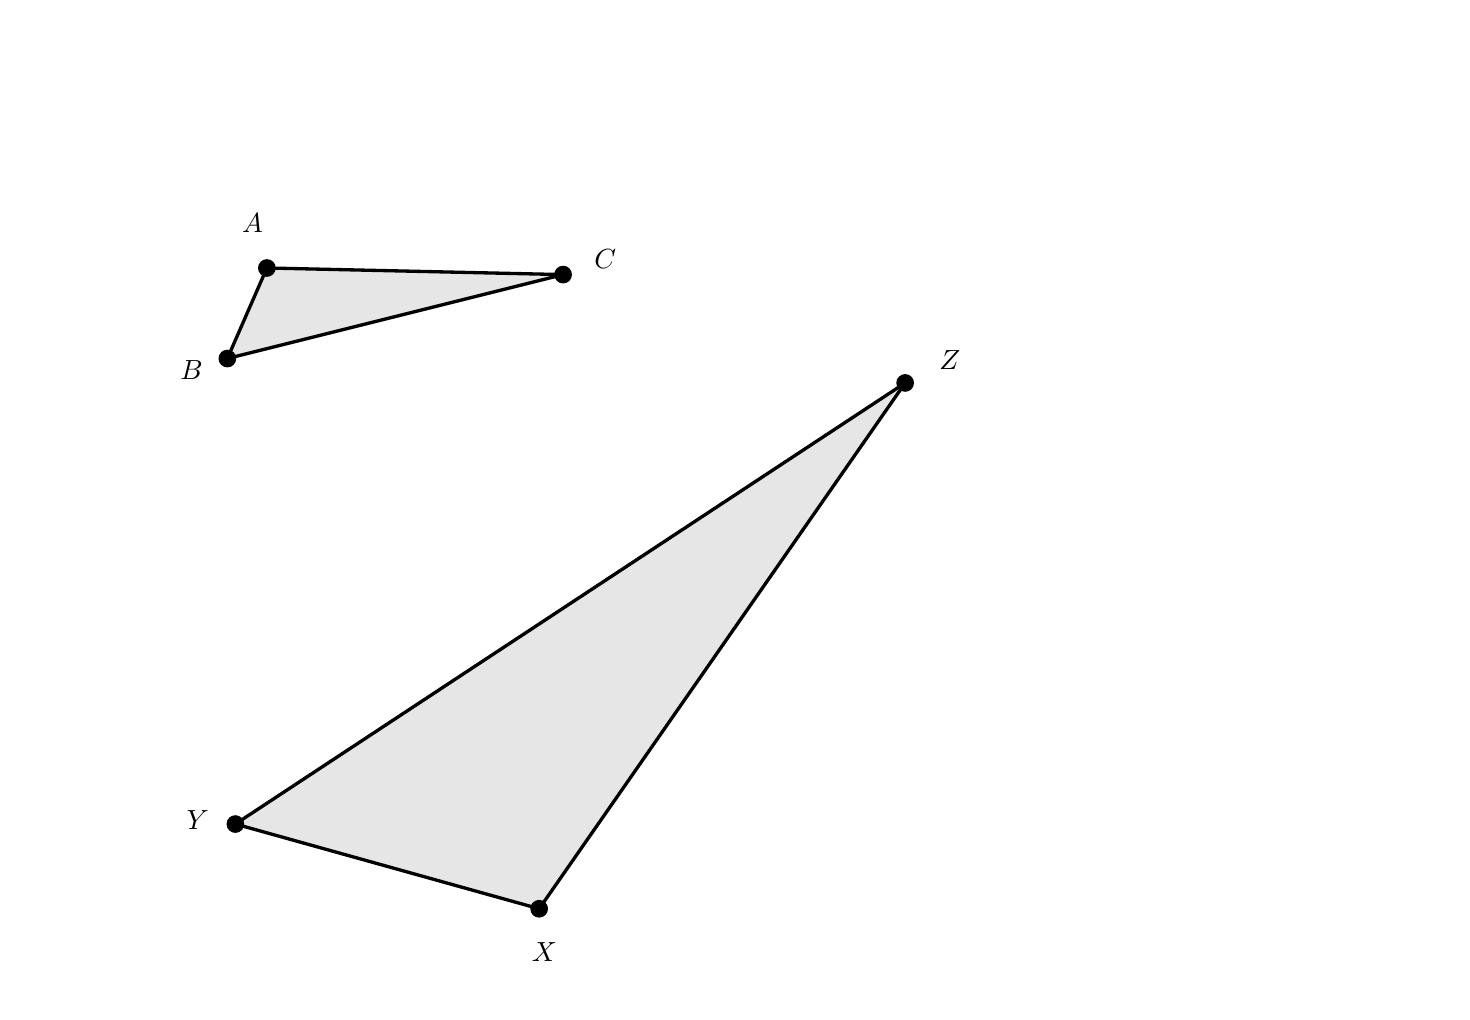
\begin{tikzpicture}[scale = 0.2]
    \clip(-20.65,-28.57) rectangle (69.12,32.66);
    \fill[line width=0pt,color=ttqqcc,fill=ttqqcc,fill opacity=0.15] (-5.46,17.4) -- (-7.97,11.65) -- (13.35,16.98) -- cycle;
    \fill[line width=0pt,color=ttqqcc,fill=ttqqcc,fill opacity=0.15] (11.83,-23.29) -- (-7.46,-17.91) -- (35.07,10.1) -- cycle;
    \draw [line width=1.2pt] (-5.46,17.4)-- (-7.97,11.65);
    \draw [line width=1.2pt] (-7.97,11.65)-- (13.35,16.98);
    \draw [line width=1.2pt] (13.35,16.98)-- (-5.46,17.4);
    \draw [line width=1.2pt] (11.83,-23.29)-- (-7.46,-17.91);
    \draw [line width=1.2pt] (-7.46,-17.91)-- (35.07,10.1);
    \draw [line width=1.2pt] (35.07,10.1)-- (11.83,-23.29);
    \begin{scriptsize}
        \normalsize
        \fill [color=black] (-7.97,11.65) circle (16pt);
        \draw[color=black] (-10.25,10.92) node {$B$};
        \fill [color=black] (13.35,16.98) circle (16pt);
        \draw[color=black] (16.03,17.99) node {$C$};
        \fill [color=black] (-5.46,17.4) circle (16pt);
        \draw[color=black] (-6.38,20.25) node {$A$};
        \fill [color=black] (11.83,-23.29) circle (16pt);
        \draw[color=black] (12.16,-26.03) node {$X$};
        \fill [color=black] (-7.46,-17.91) circle (16pt);
        \draw[color=black] (-9.85,-17.63) node {$Y$};
        \fill [color=black] (35.07,10.1) circle (16pt);
        \draw[color=black] (37.91,11.58) node {$Z$};
    \end{scriptsize}
\end{tikzpicture}
    \end{figure}
    \vspace*{\fill}
\end{section-exercise}